\documentclass{article}
\usepackage[utf8]{inputenc}
\usepackage{listings}
\usepackage{multimedia} % to embed movies in the PDF file
\usepackage{graphicx}
\usepackage{comment}
\usepackage[english]{babel}
\usepackage{amsmath}
\usepackage{amsfonts}
\usepackage{wrapfig}
\usepackage{multirow}
\usepackage{verbatim}
\usepackage{float}
\usepackage{cancel}
\usepackage{caption}
\usepackage{subcaption}
\usepackage{/home/cade/Homework/latex-defs}
\usepackage{/home/cade/Homework/jlcode}
\DeclareUnicodeCharacter{1F438}{{\coloremoji{🐸}}}


\title{AMATH 586 Homework 3}
\author{Cade Ballew \#2120804}
\date{May 6, 2022}

\begin{document}
	
\maketitle
	
\section{Problem 1}
Consider a consistent and zero-stable LMM
\begin{align*}
	\sum_{j=0}^r \alpha_j U^{n+j} = k \sum_{j=0}^r \beta_j f(U^{n+j}).
\end{align*}
and define the characteristic polynomial $\pi(\xi;z) = \rho(\xi) - z \sigma(\xi)$.\\
From (5.48), we have that a LMM is consistent iff 
\[
\sum_{j=0}^{r}\alpha_j=0,\quad\sum_{j=0}^{r}j\alpha_j=\sum_{j=0}^r\beta_j. 
\]
We can then see from the definition that
\[
\pi(1;0)=\rho(1)=\sum_{j=0}^{r}\alpha_j=0
\]
if the LMM is consistent. \\
If our method is both consistent and zero-stable, then we know from consistency that $\rho(1)=0$. However, zero-stability tells us that any roots of $\rho$ with modulus 1 must have multiplicity 1. Thus, since $\rho$ is a polynomial, we must be able to write 
\[
\rho(\xi)=(\xi-1)g(\xi)
\]
where $g$ is a polynomial such that $g(1)\neq0$. Then,
\[
\rho'(\xi)=g(\xi)+(\xi-1)g'(\xi),
\]
so 
\[
\rho'(1)=g(1)\neq0.
\]
Now, we assume zero-stability and consistency and suppose $\xi = 1 + \eta(z)$ for $z$ near zero so that $\pi(\xi;z) = \pi(1 + \eta(z);z) = 0$. Then, taking the derivative with respect to $z$ of both sides of this equation, 
\begin{align*}
\frac{\partial \pi}{\partial z}=\rho'(1+\eta(z))\eta'(z)-\sigma(1+\eta(z))-z\sigma'(1+\eta(z))\eta'(z)=0.
\end{align*}
This lets us find that 
\[
\eta'(z)=\frac{\sigma(1+\eta(z))}{\rho'(1+\eta(z))-z\sigma'(1+\eta(z))}.
\]
Taking $\eta(0)=0$, %maybe explain why; implict function theorem 
\[
\eta'(0)=\frac{\sigma(1)}{\rho'(1)}.
\]
Now, note that
\[
\rho'(\xi)=\sum_{j=1}^rj\alpha_j\xi^{j-1},
\]
so consistency gives that
\[
\rho'(1)=\sum_{j=1}^rj\alpha_j=\sum_{j=0}^r\beta_j=\sigma(1).
\]
Thus, we find that $\eta'(0)=1$. We can see this implies that there must be an interval $(0,\epsilon]$ for some small $\epsilon > 0$ that does not lie in the absolute stability region $S$ by letting $\epsilon > 0$ be small. Then, the mean value theorem gives that
\[
\eta(\epsilon)-\eta(0)=\eta'(\zeta)(\epsilon-0)=\eta'(\zeta)\epsilon
\]
for some $\zeta\in(0,\epsilon)$. If $\epsilon$ is sufficiently small, then continuity gives that $\eta'(\zeta)\approx \eta'(0)=1$ and $\eta'(\zeta)>0$. Then, 
\[
\xi=1+\eta(\epsilon)=1+\eta'(\zeta)\epsilon>1
\]
meaning that the root condition is violated and $\epsilon$ (or any nonnegative values less than it) cannot fall in the absolute stability region. We could also observe this by Taylor expanding $\eta$ as
\[
\eta(z)=\eta(0)+\eta'(0)z+\oo(z)=z+\oo(z)
\]
where $z>0$ is sufficiently close to $0$ and using the reverse triangle inequality to write
\[
|\xi|=|1+z+\oo(z)|\geq|1+z|-|\oo(z)|=1+z-|\oo(z)|>1
\]
as $z\gg\oo(z)$.

\section{Problem 2}
Consider the system of ODEs
\begin{align*}
	\begin{bmatrix} u_1'(t) \\ u_2'(t) \\ u_3'(t) \\ u_4'(t) \end{bmatrix} = \begin{bmatrix} u_4(t) - \mu u_3(t) + \lambda g(u_1(t) + u_2(t))\\
		\mu u_3(t) - u_4(t) +  \lambda g(u_1(t) + u_2(t))\\
		- \sigma u_4(t) \\
		\sigma  u_3(t) \end{bmatrix}, \quad g(u) = u (1-u)^2, \quad \lambda > 0, ~ \sigma, \mu \in \mathbb R.
\end{align*}
To solve for $u_3(t),u_4(t)$ in terms of $u_3(0) = \eta_3,u _4(0) = \eta_4$, we note that
\[
\begin{pmatrix}
	u_3'(t)\\u_4'(t)
\end{pmatrix}=\begin{pmatrix}
-\sigma u_4(t)\\\sigma u_3(t)
\end{pmatrix}=\begin{pmatrix}
0 &-\sigma\\ \sigma &0
\end{pmatrix}\begin{pmatrix}
u_3(t)\\u_4(t)
\end{pmatrix}
\]
and define 
\[
A=\begin{pmatrix}
	0 &-\sigma\\ \sigma &0
\end{pmatrix}.
\]
We compute the matrix exponential by diagonalizing
\[
A = \begin{pmatrix}
-i &i\\ 1 &1
\end{pmatrix}\begin{pmatrix}
-i\sigma &0\\ 0 &i\sigma
\end{pmatrix}\begin{pmatrix}
i/2 &1/2\\-i/2 &1/2
\end{pmatrix},
\]
so 
\begin{align*}
e^{tA}&=\begin{pmatrix}
	-i &i\\ 1 &1
\end{pmatrix}\begin{pmatrix}
	e^{-i\sigma t} &0\\ 0 &e^{i\sigma t}
\end{pmatrix}\begin{pmatrix}
	i/2 &1/2\\-i/2 &1/2
\end{pmatrix}=\begin{pmatrix}
-ie^{-i\sigma t} &ie^{i\sigma t}\\ e^{-i\sigma t} &e^{i\sigma t}
\end{pmatrix}\begin{pmatrix}
i/2 &1/2\\-i/2 &1/2
\end{pmatrix}\\&=
\begin{pmatrix}
	\frac{1}{2}(e^{-i\sigma t}+e^{i\sigma t}) &\frac{i}{2}(e^{i\sigma t}-e^{-i\sigma t})\\
	\frac{i}{2}(e^{-i\sigma t}-e^{i\sigma t}) &\frac{1}{2}(e^{-i\sigma t}+e^{i\sigma t})
\end{pmatrix}=\begin{pmatrix}
\cos(\sigma t) &-\sin(\sigma t)\\
\sin(\sigma t) &\cos(\sigma t)
\end{pmatrix}.
\end{align*}
Thus,
\[
\begin{pmatrix}
	u_3(t)\\u_4(t)
\end{pmatrix}=e^{tA}\eta=\begin{pmatrix}
\eta_3\cos(\sigma t)-\eta_4\sin(\sigma t)\\
\eta_3\sin(\sigma t)+\eta_4\cos(\sigma t)
\end{pmatrix}.
\]
Now, we define $w(t)=u_1(t)-u_2(t)$ and subtract the first two equations of our original system to find that 
\begin{align*}
w'(t)&=u_1'(t)-u_2'(t)=(u_4(t) - \mu u_3(t) + \lambda g(u_1(t) + u_2(t)))-(\mu u_3(t) - u_4(t) +  \lambda g(u_1(t) + u_2(t)))\\&=
2(u_4(t)-\mu u_3(t))=2(\eta_3\sin(\sigma t)+\eta_4\cos(\sigma t)-\mu\eta_3\cos(\sigma t)+\mu\eta_4\sin(\sigma t)).
\end{align*}
We solve this ODE by integrating both sides to get
\[
w(t)=\frac{2}{\sigma}(-\eta_3\cos(\sigma t)+\eta_4\sin(\sigma t)-\mu\eta_3\sin(\sigma t)-\mu\eta_4\cos(\sigma t))+C. 
\]
For any fixed choice of $u_1(0) = \eta_1,u_2(0) = \eta_2,u_3(0) = \eta_3,u _4(0) = \eta_4$, we have the boundary condition $w(0)=\eta_1-\eta_2$ which gives that
\[
\eta_1-\eta_2=\frac{2}{\sigma}(-\eta_3-\mu\eta_4)+C,
\]
so
\[
w(t)=\frac{2}{\sigma}(-\eta_3\cos(\sigma t)+\eta_4\sin(\sigma t)-\mu\eta_3\sin(\sigma t)-\mu\eta_4\cos(\sigma t)+\eta_3+\mu\eta_4)+\eta_1-\eta_2.
\]
This is clearly bounded as $t\to\infty$ as by the triangle inequality 
\begin{align*}
|w(t)|&\leq \frac{2}{|\sigma|}(|\eta_3\cos(\sigma t)|+|\eta_4\sin(\sigma t)|+|\mu\eta_3\sin(\sigma t)|+|\mu\eta_4\cos(\sigma t)|+|\eta_3|+|\mu\eta_4|)+|\eta_1|+|\eta_2|\\&\leq
\frac{2}{|\sigma|}(|\eta_3|+|\eta_4|+|\mu\eta_3|+|\mu\eta_4|+|\eta_3|+|\mu\eta_4|)+|\eta_1|+|\eta_2|,
\end{align*}
so $|w(t)|$ is bounded by initial conditions that are fixed (finite) and constant $\frac{2}{|\sigma|}$.\\
Now, consider $v(t)=u_1(t)+u_2(t)$. We add the first two equations of our system to find that
\begin{align*}
	v'(t)&=u_1'(t)+u_2'(t)=(u_4(t) - \mu u_3(t) + \lambda g(u_1(t) + u_2(t)))+(\mu u_3(t) - u_4(t) +  \lambda g(u_1(t) + u_2(t)))\\&=
	2\lambda g(u_1(t) + u_2(t))=2\lambda g(v(t))=2\lambda v(t)(1-v(t))^2.
\end{align*}
Note that $v(0)=u_1(0)+u_2(0)=\eta_1+\eta_2$, so if $0<\eta_1+\eta_2<1$, $0<v(0)<1$. This implies that $v'(0)>0$ as $\lambda>0$, so $v(t)$ will increase initially and continue to do so until $v(t)=1$ as $2\lambda v(t)(1-v(t))^2>0$ for $\lambda\in (0,1)$. Once $v(t)=1$, $2\lambda v(t)(1-v(t))^2=0$, so $v'(t)=0$ for all $t$ after $v(t)=1$ is first achieved (This is an absorbing state). Thus, $|v(t)|\leq1$ as $t\to\infty$ meaning that $v(t)$ is bounded. \\
Since $v(t),w(t)$ are both bounded as $t\to\infty$, both $u_1(t)$ and $u_2(t)$ are bounded as well as
\[
|u_1(t)|=|\half(w(t)+v(t))|\leq\half(|w(t)|+|v(t)|)
\]
and
\[
|u_1(t)|=|\half(w(t)-v(t))|\leq\half(|w(t)|+|v(t)|).
\]

\section{Problem 3}
Now, we consider the system of ODEs from problem 2 and take $u_1(0) = 0.1, ~u_2(0) = 0.1, ~u_3(0) = 0, u_4(0) = 0.1$ and $\lambda = 10$, $\sigma = 200$, $\mu = 100$. Using Julia, we first solve solve this problem with trapezoid with $k = 0.0001$ which we treat as the true solution. This is displayed in the following plot which has a final time of $T=20$. \\
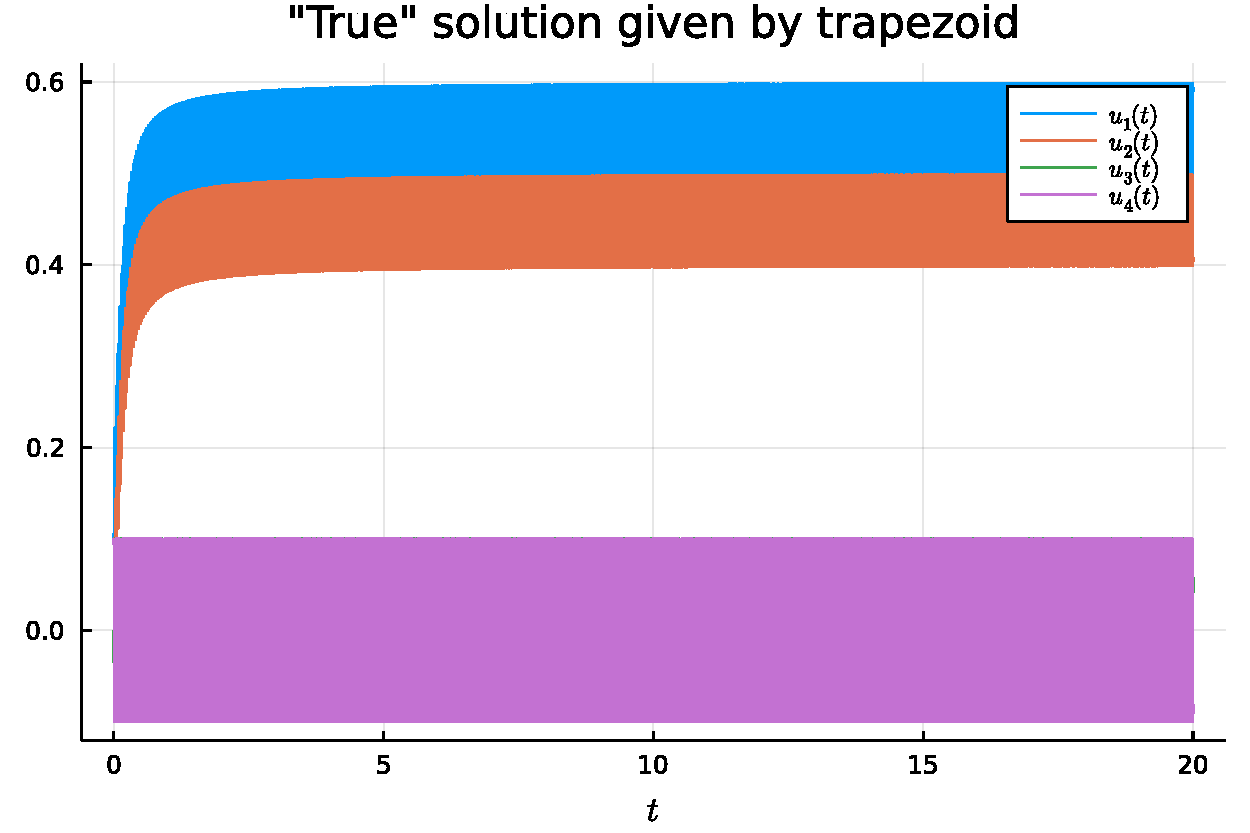
\includegraphics[scale=0.5]{trap.pdf}\\
Note that the apparent shaded regions are due to heavy oscillation and is why $u_4(t)$ appears superimposed over $u_3(t)$. The Jacobian of our system is given by
\[
J_u=\begin{pmatrix}
\lambda g'(u_1+u_2) &\lambda g'(u_1+u_2) &-\mu &1\\
\lambda g'(u_1+u_2) &\lambda g'(u_1+u_2) &\mu &-1\\
0 &0 &0 &-\sigma\\
0 &0 &\sigma &0
\end{pmatrix}.
\]
The following is a plot of the eigenvalues sorted by imaginary part of the Jacobian at each timestep of this solution\\
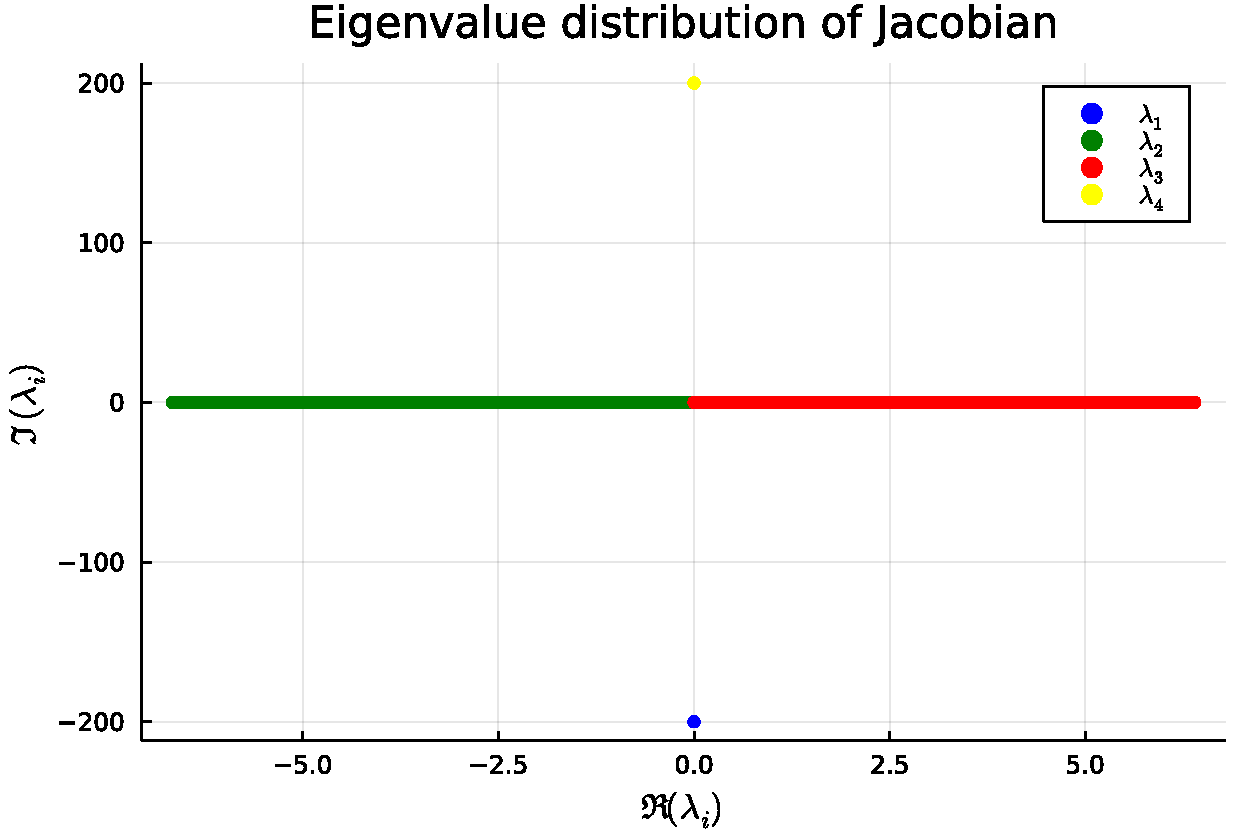
\includegraphics[scale=0.5]{eigvals.pdf}\\
Now, we take $k=0.001$ and solve the system with forward Euler which yields the following plot. \\
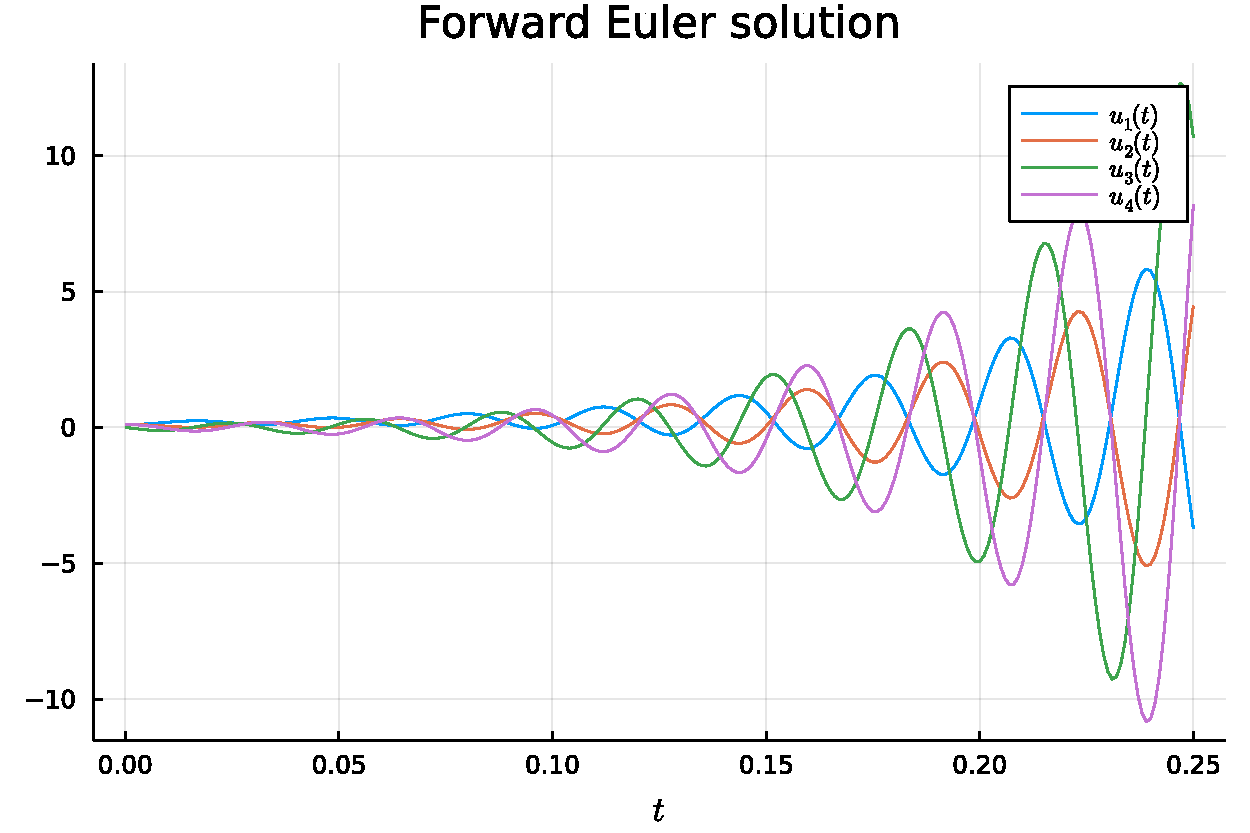
\includegraphics[scale=0.5]{fe.pdf}\\
Notice how instability begins almost immediately and our values are an order of magnitude removed from the true values by $t=0.25$. \\
Now, we again take $k=0.001$ and solve the system with leapfrog which yields the following plot. \\
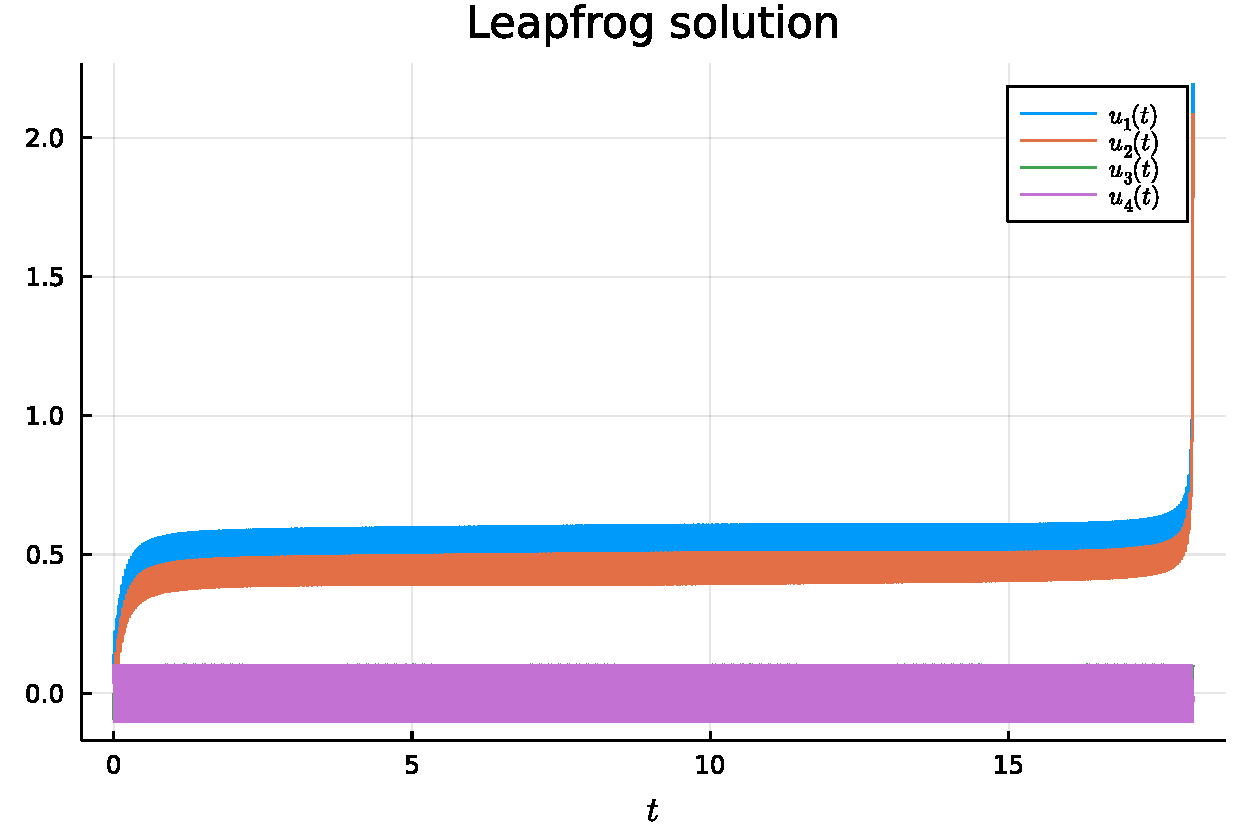
\includegraphics[scale=0.5]{lf.pdf}\\
This time, our solution does become unstable but only around $t=18$ which is significantly better than forward Euler.\\
The accuracy of these methods can be explained by how well their regions of stability capture the eigenvalues of our Jacobian. Since forward Euler's region of stability is a disk of unit radius centered at $-1$, it is only able to capture the eigenvalues on the imaginary axis with a sufficiently small timestep. Leapfrog also captures the eigenvalues poorly as its stability region is entirely on the imaginary axis from $-i$ to $i$, so we again need to choose a sufficiently small timestep to ensure stability and the eigenvalues on the real axis are only captured when they are zero.  On the other hand, trapezoid's stability region is the left halfplane including the imaginary axis, so the eigenvalues on the imaginary axis are always captured (regardless of stepsize) along with whichever real eigenvalue is nonpositive, meaning that 3 out 4 four eigenvalues are always captured. Thus, we can choose our stepsize to maximize accuracy rather than having to choose one which ensures stability.\\
See Appendix A for the Julia code utilized in this problem. 

\section{Problem 4}
Using Julia, we plot the absolute stability region for the TR-BDF2 method (8.6) by recalling from homework 2 that 
\[
R(z)=\frac{12+5z}{(3-z)(4-z)}.
\]
We obtain the following plot in which the yellow denotes the stablity region. \\
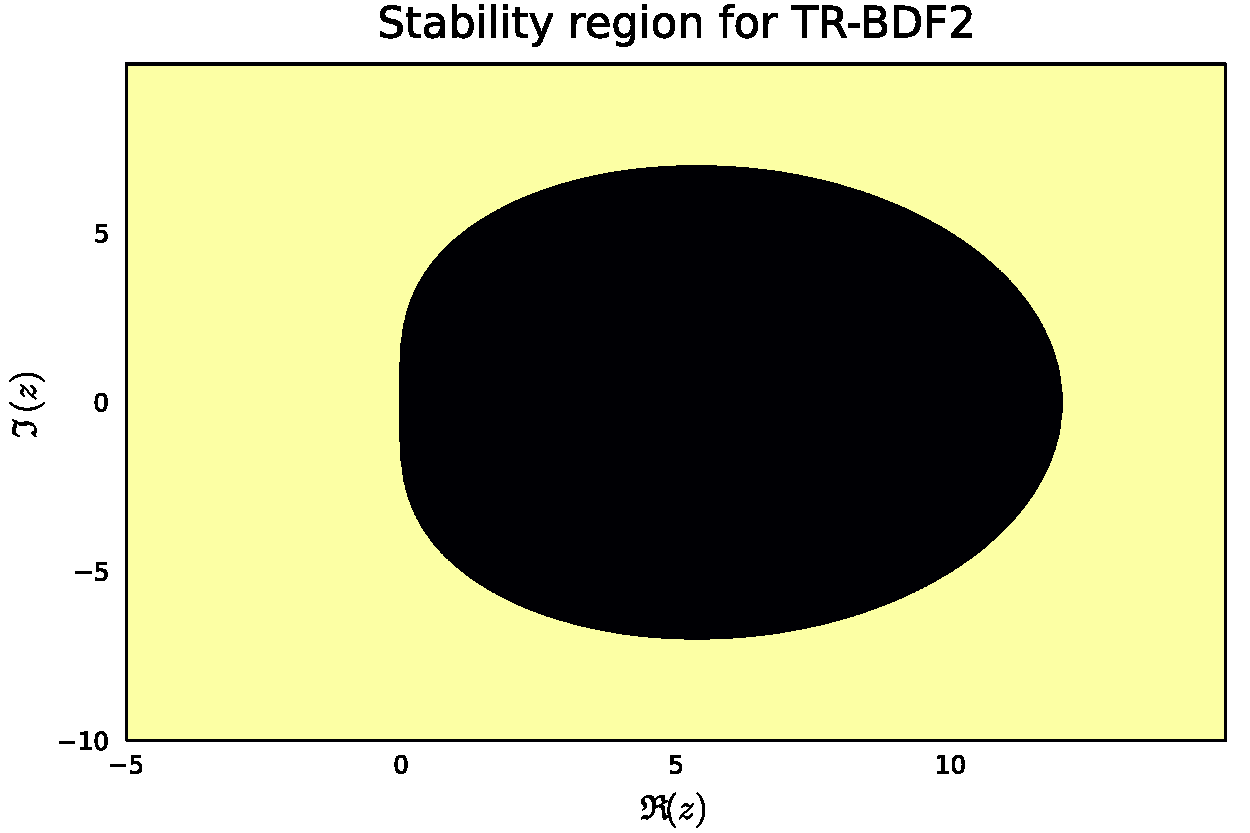
\includegraphics[scale=0.5]{trbdf.pdf}\\
See Appendix A for the relevant code. \\
To show that this method is A-stable, let $z=iy$ where $y\in\real$. Then,
\begin{align*}
|R(z)|^2=\frac{|12+5iy|^2}{|(3-iy)(4-iy)|^2}=\frac{|12+5iy|^2}{|(12+y^2)-7iy|^2}=\frac{144+25y^2}{144+24y^2+y^4+49y^2}.
\end{align*}
Thus, $|R(iy)|\leq1$ iff $144+25y^2\leq144+73y^2+y^4$ which holds iff $y^4+48y^2=y^2(y^2+48)\geq0$. This clearly holds for any $y\in\real$, so we must have that $|R(z)|\leq1$ on the imaginary axis. Now, we note that $R$ is analytic in the left halfplane (as its only singularities are at $z=3,4$) and that $R(z)\to0$ as $z\to\infty$. We apply the maximum modulus principle (for rational functions) which gives that the modulus of $R$ in the closure of the left halfplane must be attained on its boundary (the imaginary axis and infinity). Since $R(z)\to0$ as $z\to\infty$, we must have that $|R(z)|$ attains its maximum in this region on the imaginary axis, so it must actually hold that $|R(z)|\leq1$ for all $z$ such that $\Re z\leq0$. Thus, the method is A-stable. \\
As we have already claimed\footnote{The denominator has a higher degree than the numerator.},
\[
\lim_{z\to\infty}|R(z)|=0,
\]
so our method is also L-stable.

\section{Problem 5}
Let $g(x)=0$ represent a system of $s$ nonlinear equations in $s$ unknowns,
so $x\in\real^s$ and $g: \real^s \to \real^s$.  A vector $\bar
x\in\real^s$ is a {\em fixed point} of $g(x)$ if 
\begin{equation}\label{a}
	\bar x = g(\bar x).
\end{equation}
One way to attempt to compute $\bar x$ is with {\em fixed point iteration}:
from some starting guess $x^0$, compute
\begin{equation}\label{b}
	x^{j+1} = g(x^j)
\end{equation}
for $j=0,~1,~\ldots$.

\subsection{Part a}
Assume that there exists a norm $\|\cdot\|$ such that $g(x)$ is
Lipschitz continuous with constant $L<1$ in a neighborhood of $\bar x$. We first need to demonstrate that a fixed point iteration that starts in this neighborhood remains in it. Namely, we assume that 
\[
\|x-\bar{x}\|<\epsilon
\]
where $\epsilon>0$ is the radius of the neighborhood and use the Lipschitz continuity to find that 
\[
\|g(x)-\bar{x}\|=\|g(x)-g(\bar{x})\|\leq L\|x-\bar{x}\|=L\epsilon<\epsilon.
\]
This means that the fixed point iteration applied to a point in the neighborhood produces a point that is also in the neighborhood. Applying this property inductively yields that all iterations of the fixed point iteration are within this neighborhood if we assume that the starting value $x^0$ is within it. With this, we can apply the Lipschitz property at each iteration. Namely, subtracting \eqref{a} from \eqref{b},
\begin{align*}
\|x^{j+1}-\bar{x}\|&=\|g(x^j)-g(\bar{x})\|\leq L\|x^j-\bar{x}\|=\|g(x^{j-1})-g(\bar{x})\|\\&\leq
L^2\|x^{j-1}-\bar{x}\|\leq\ldots\leq L^{j+1}\|x^0-\bar{x}\|
\end{align*}
for $j=0,1,\ldots$. Thus,
\[
\lim_{j\to\infty}\|x^j-\bar{x}\|=\lim_{j\to\infty}L^j\|x^0-\bar{x}\|=0
\]
since $L<1$. Thus, it must hold that
\[
\lim_{j\to\infty}x^j=\bar{x},
\]
so the fixed point iteration converges. 

\subsection{Part b}
Suppose $g(x)$ is differentiable and let $D_xg(x)$ be the $s\times s$
Jacobian matrix. Consider some $x^*$ which is within a neighborhood of $\bar{x}$ required for Lipschitz continuity and Taylor expansion. Then,
\[
g(x^*)=g(\bar{x})+D_xg(\bar{x})(x^*-\bar{x})+\oo(\|x^*-\bar{x}\|),
\]
so
\[
D_xg(\bar{x})(x^*-\bar{x})=g(x^*)-g(\bar{x})+\oo(\|x^*-\bar{x}\|),
\]
and 
\begin{align*}
\|D_xg(\bar{x})(x^*-\bar{x})\|\leq\|g(x^*)-g(\bar{x})\|+\oo(\|x^*-\bar{x}\|)\leq L\|x^*-\bar{x}\|+\oo(\|x^*-\bar{x}\|).
\end{align*}
Then,
\[
\frac{\|D_xg(\bar{x})(x^*-\bar{x})\|}{\|x^*-\bar{x}\|}\leq L+\oo(1).
\]
Since this must hold for all $x^*$ in a certain neighborhood, it must hold that 
\[
\max_{\|x^*-\bar{x}\|=\delta}\frac{\|D_xg(\bar{x})(x^*-\bar{x})\|}{\|x^*-\bar{x}\|}\leq L+\oo(1).
\]
where $\delta>0$ is less than the radius of our neighborhood. However, we can simply let $y=(x^*-\bar{x})/\delta$ to get that 
\[
\max_{\|y\|=1}\|D_xg(\bar{x})y\|\leq L+\oo(1).
\]
The LHS is the definition of the operator norm, so taking the limit of both sides as $\delta\to0$, we find that 
\[
\|D_xg(\bar{x})\|\leq L<1.
\]
It also holds that for any operator norm,
\[
\rho(A)\leq\|A\|
\]
where $A$ is a matrix and $\rho$ is its spectral radius, so we must also have that 
\[
\rho(D_xg(\bar{x}))<1.
\]

\subsection{Part c}
Consider a predictor-corrector method consisting
of forward Euler as the predictor and backward Euler as the corrector, and
suppose we make $N$ correction iterations, i.e., we set
\begin{tabbing}
	xxxxxxxxx\=xxxx\=\kill\\
	\>$\hat U^0 = U^n + kf(U^n)$\\
	\>for $j = 0,~1,~\ldots,~N-1$\\
	\>\>$\hat U^{j+1} = U^n + kf(\hat U^j)$\\
	\>\>end\\
	\>$U^{n+1} = \hat U^N$.\\
\end{tabbing}
To find the stability region for this method, we consider the method applied for $f(U)=\lambda U$. Using induction, we prove that 
\[
\hat{U}^N=\left(\sum_{j=0}^{N+1}z^j\right)U^n
\]
where $z=k\lambda$. As a base case where $N=0$, we find that 
\[
\hat{U}^0=U^n+kf(U^n)=U^n+k\lambda U^n=(1+z)U^n.
\]
Now, say that the formula holds for $N=\ell-1$. Then,
\[
\hat{U}^\ell=U^n+kf(\hat{U}^{\ell-1})=U^n+k\lambda\left(\sum_{j=0}^{\ell}z^j\right)U^n=\left(1+\sum_{j=0}^{\ell}z^{j+1}\right)U^n=\left(\sum_{j=0}^{\ell+1}z^j\right)U^n
\]
after reindexing. Thus, the formula holds for all $N\in\mathbb{N}$ by induction. Since $U^{n+1}=\hat{U}^N$, 
\[
U^{n+1}=\left(\sum_{j=0}^{N+1}z^j\right)U^n,
\]
so
\[
R(z)=\sum_{j=0}^{N+1}z^j.
\]
Using Julia, we plot the stability region corresponding to $|R(z)|\leq1$ for $N=2,~5,~10,~20,~50$ and obtain the following plots. \\
\begin{figure}[H]
	\centering
	\begin{subfigure}{0.495\linewidth}
		\centering
		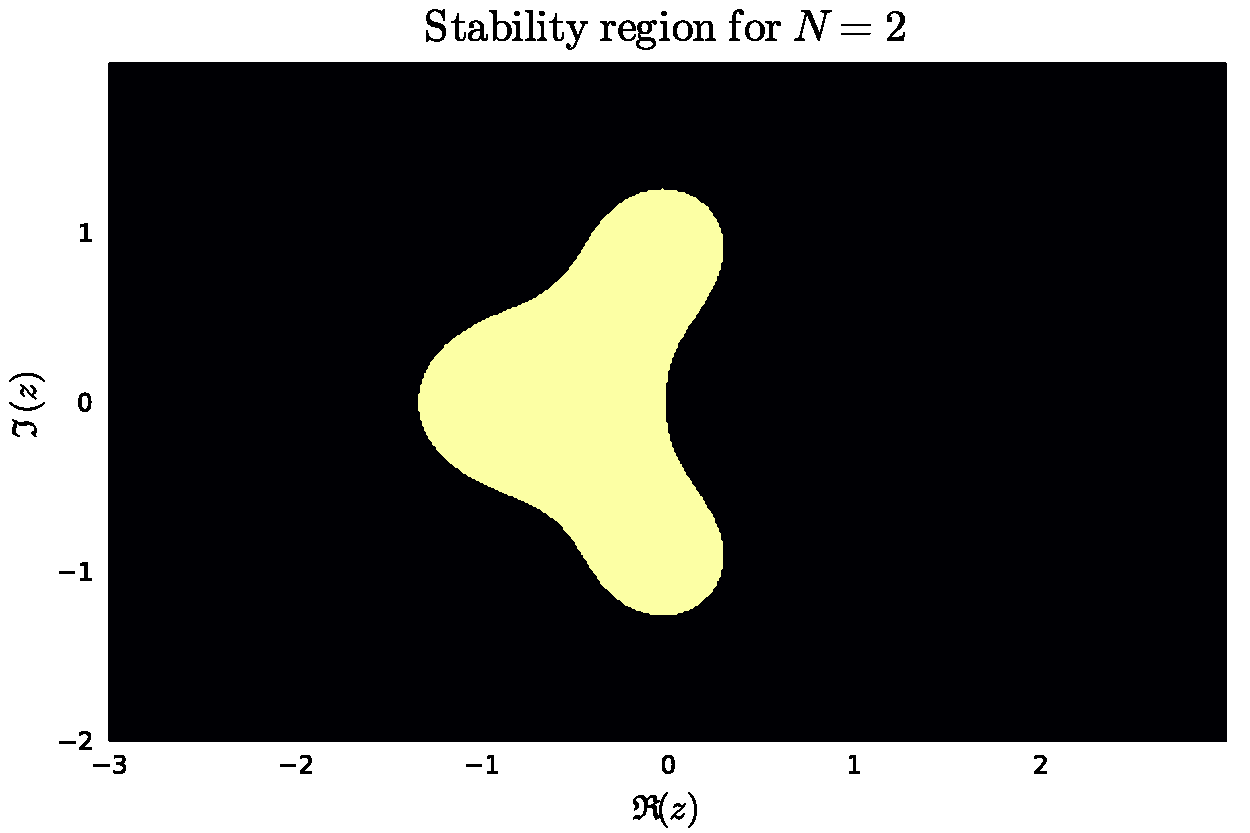
\includegraphics[width=\linewidth]{N2.pdf}
	\end{subfigure}
	\begin{subfigure}{0.495\linewidth}
		\centering
		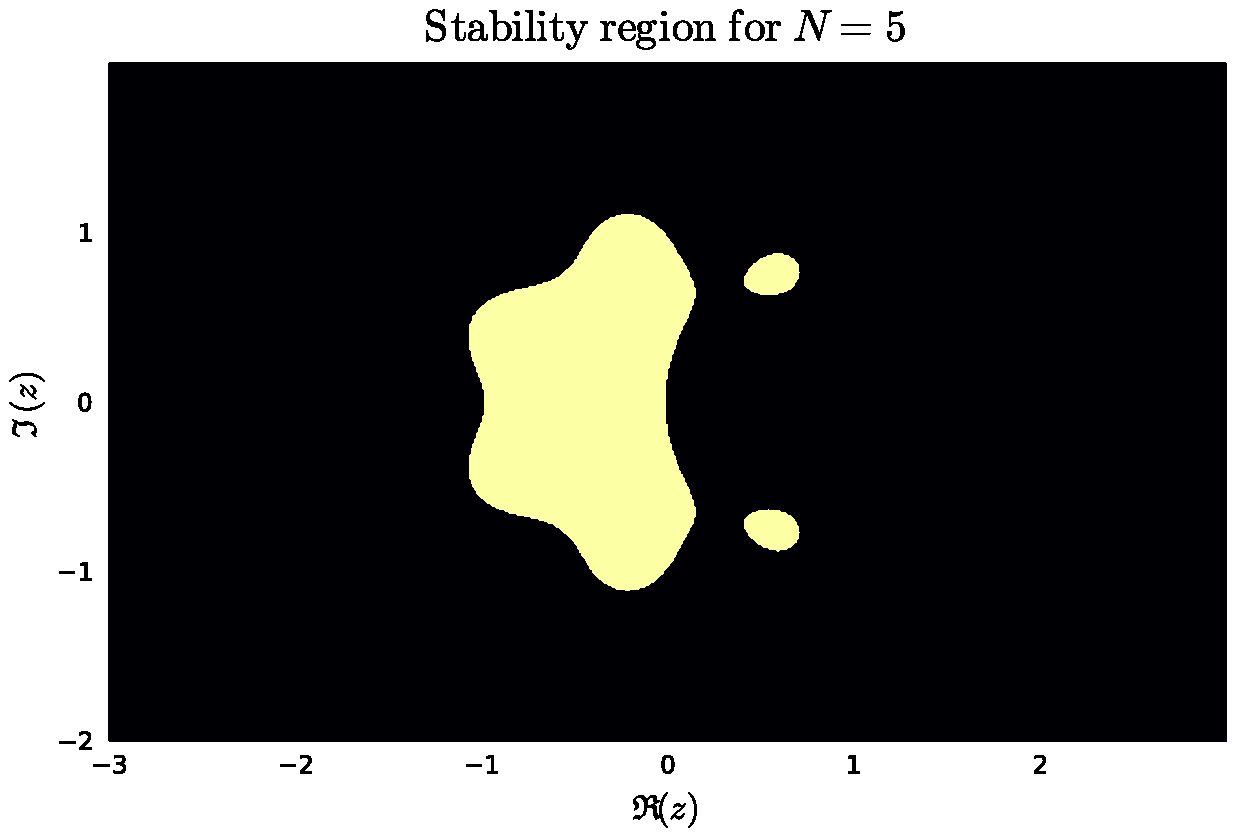
\includegraphics[width=\linewidth]{N5.pdf}
	\end{subfigure}
	\begin{subfigure}{0.495\linewidth}
		\centering
		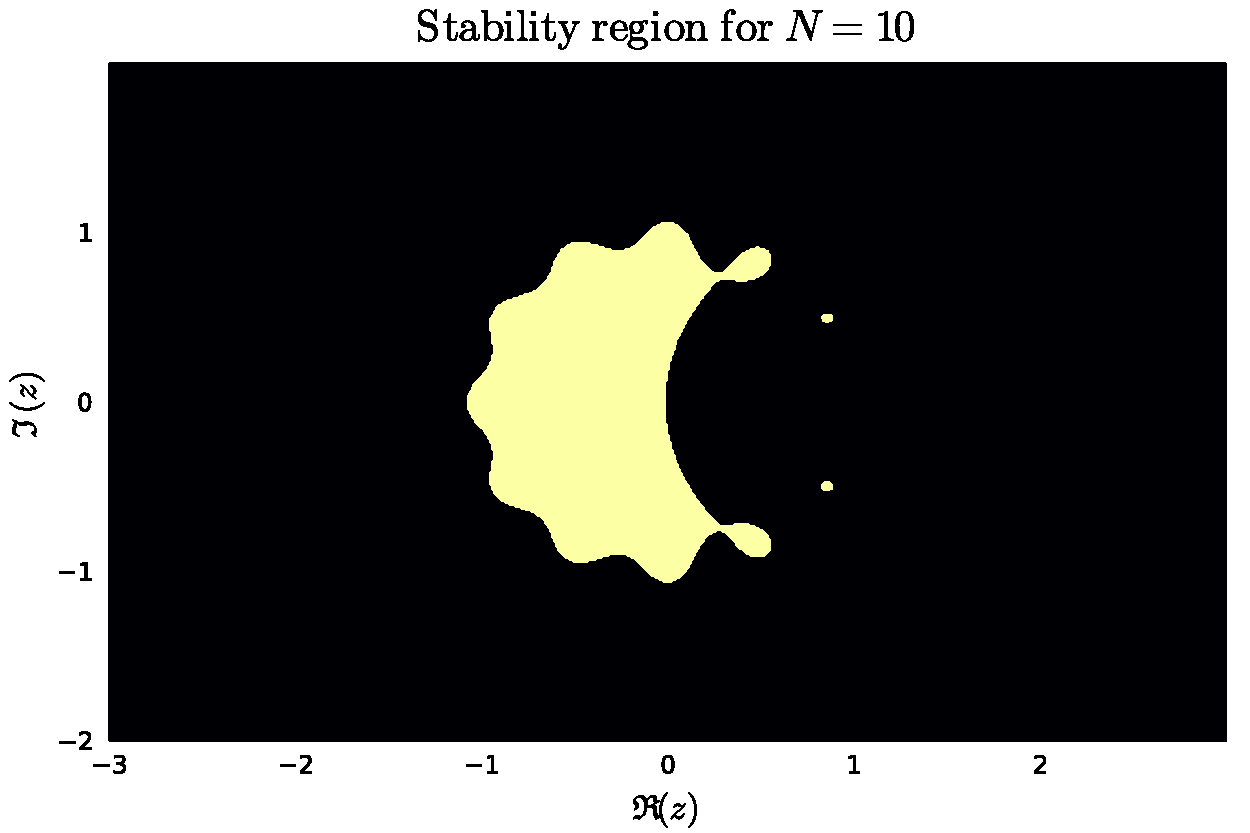
\includegraphics[width=\linewidth]{N10.pdf}
	\end{subfigure}
	\begin{subfigure}{0.495\linewidth}
		\centering
		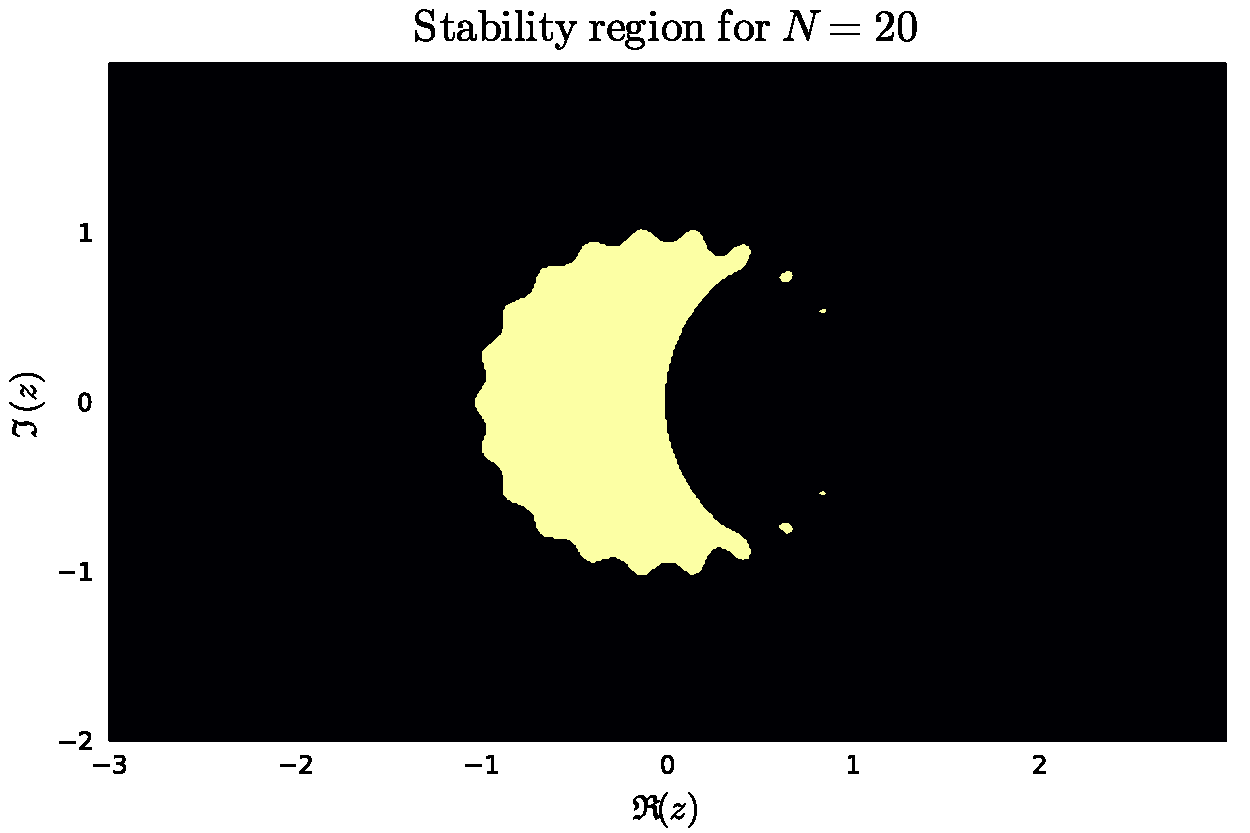
\includegraphics[width=\linewidth]{N20.pdf}
	\end{subfigure}
\end{figure}
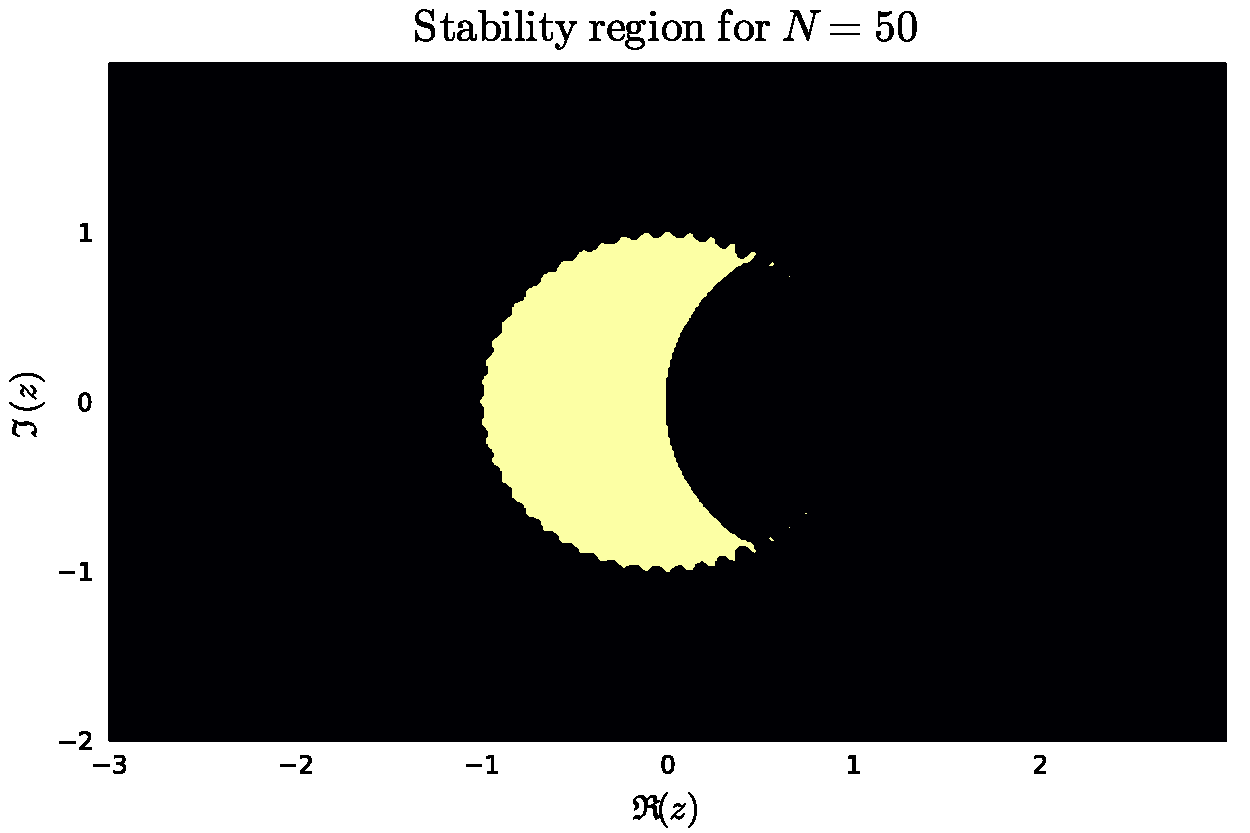
\includegraphics[scale=0.5]{N50.pdf}

\subsection{Part d}
Consider $g(U)=U^n+kf(U)$ as a fixed point iteration\footnote{Note that this is the iteration being used in part c.}. Then, its Jacobian is given by
\[
D_ug(u)=kf'(u)
\] 
where $f'(u)$ denotes the Jacobian of $f$. If we let $\lambda_{\text{max}}$ denote the eigenvalue of $f'(u)$ with maximum modulus, then
\[
\rho(D_ug(u))=\rho(kf'(u))=|k|\rho(f'(u))=|k||\lambda_{\text{max}}|=|k\lambda_{\text{max}}|.
\]
If for some eigenvalue $\lambda$ of $f'(u)$ $|k\lambda|\geq1$, then $|k\lambda_{\text{max}}|\geq1$ meaning that $\rho(D_ug(u))\geq1$. Then, the contrapositive of part b implies that the condition of part a cannot hold, meaning that the fixed point iteration may not hold. Thus, we can only expect convergence when $|k\lambda|<1$. 

\subsection{Part e}
From part d, we expect that the stability region only includes $z$ such that $|z|<1$. This suggests that the stability region should be the intersection of the stability region for backwards Euler with this disk which does appear to be what our region is converging to as $N\to\infty$.

\section{Problem 6}
Consider the matrix $M_r = I - r T$ where $T$ is the $m\times m$ matrix.
\begin{align*}
	T = \begin{bmatrix}
		-2 & 1 \\
		1 & -2 & 1 \\
		& 1 &-2 & \ddots\\
		& &\ddots & \ddots & 1\\
		&&& 1 & -2 \end{bmatrix}
\end{align*}
and $r \geq 0$. Because T is a tridiagonal symmetric Toeplitz matrix, its eigenvalues are given by (C.22) as 
\[
\lambda_j=-2+2\cos(j\pi h)
\]
for $j=1,\ldots,m$ where $h=\frac{1}{m+1}$. Then, the eigenvalues of $M_r$ are given by
\[
1-r\lambda_j=1-r(-2+2\cos(j\pi h))=(1+2r)-2r\cos\left(\frac{j\pi}{m+1}\right)
\]
for $j=1,\ldots,m$. Since $r\geq0$ and $\cos\left(\frac{j\pi}{m+1}\right)\leq1$,
\[
1-r\lambda_j\geq(1+2r)-2r=1>0,
\]
so it must hold that all eigenvalues of $M_r$ are positive for any $r\geq0$. This means that $M_r$ is invertible for any $r\geq0$, so the largest value of $c$ such that $M_r$ is invertible for all $ r \in [0,c)$ is $c=\infty$.

\section{Appendix A}
The following Julia code is used for Problem 3.
\jlinputlisting{Problem3.jl}
The following Julia code is used for Problem 4.
\jlinputlisting{Problem4.jl}
The following Julia code is used for Problem 5.
\jlinputlisting{Problem5.jl}

\end{document}
